\subsection{Ontology}
\label{subsec_method_ontology}

As described in the previous section, different data sources with different data formats were used. 
To create a unified dataset and therefore enable simple querying over all data, a unified ontology was defined.


The following resources, defined by the dataset, were used in the system. 
In most cases a corresponding dbpedia entity exists and thus was used.
If no dbpedia entity was present, freebase entities or newly defined ones were used.

\begin{itemize}
\item Movie: dbpedia-owl:Film
\item Award: dbpedia-owl:Award
\item MoviePerson: dbpedia-owl:Person
\item Character: freebase:film/performance
\item Aka (also known as): aka
\item ReleaseInfo: releaseInfo

\end{itemize}

A MoviePerson can have multiple sub-types of dbpedia-owl:Person, depending on the jobs the person had in any movies they worked on. 
As shown in Figure \ref{fig_ontology} a distinction between e.g. director, writer, producer was made.
Relations between the listed resources are also shown in Figure \ref{fig_ontology}.

%dbpedia-owl:Actor,
%dbpedia-owl:director,
%dbpedia-owl:Writer,
%dbpedia-owl:producer,
%dbpedia-owl:coProducer,
%dbpedia-owl:makeUpArtist,
%dbpedia-owl:costumeDesigner,
%dbpedia-owl:specialEffects,
%dbpedia-owl:setDesigner,
%dbpedia-owl:storyEditor


\begin{figure}[h!]
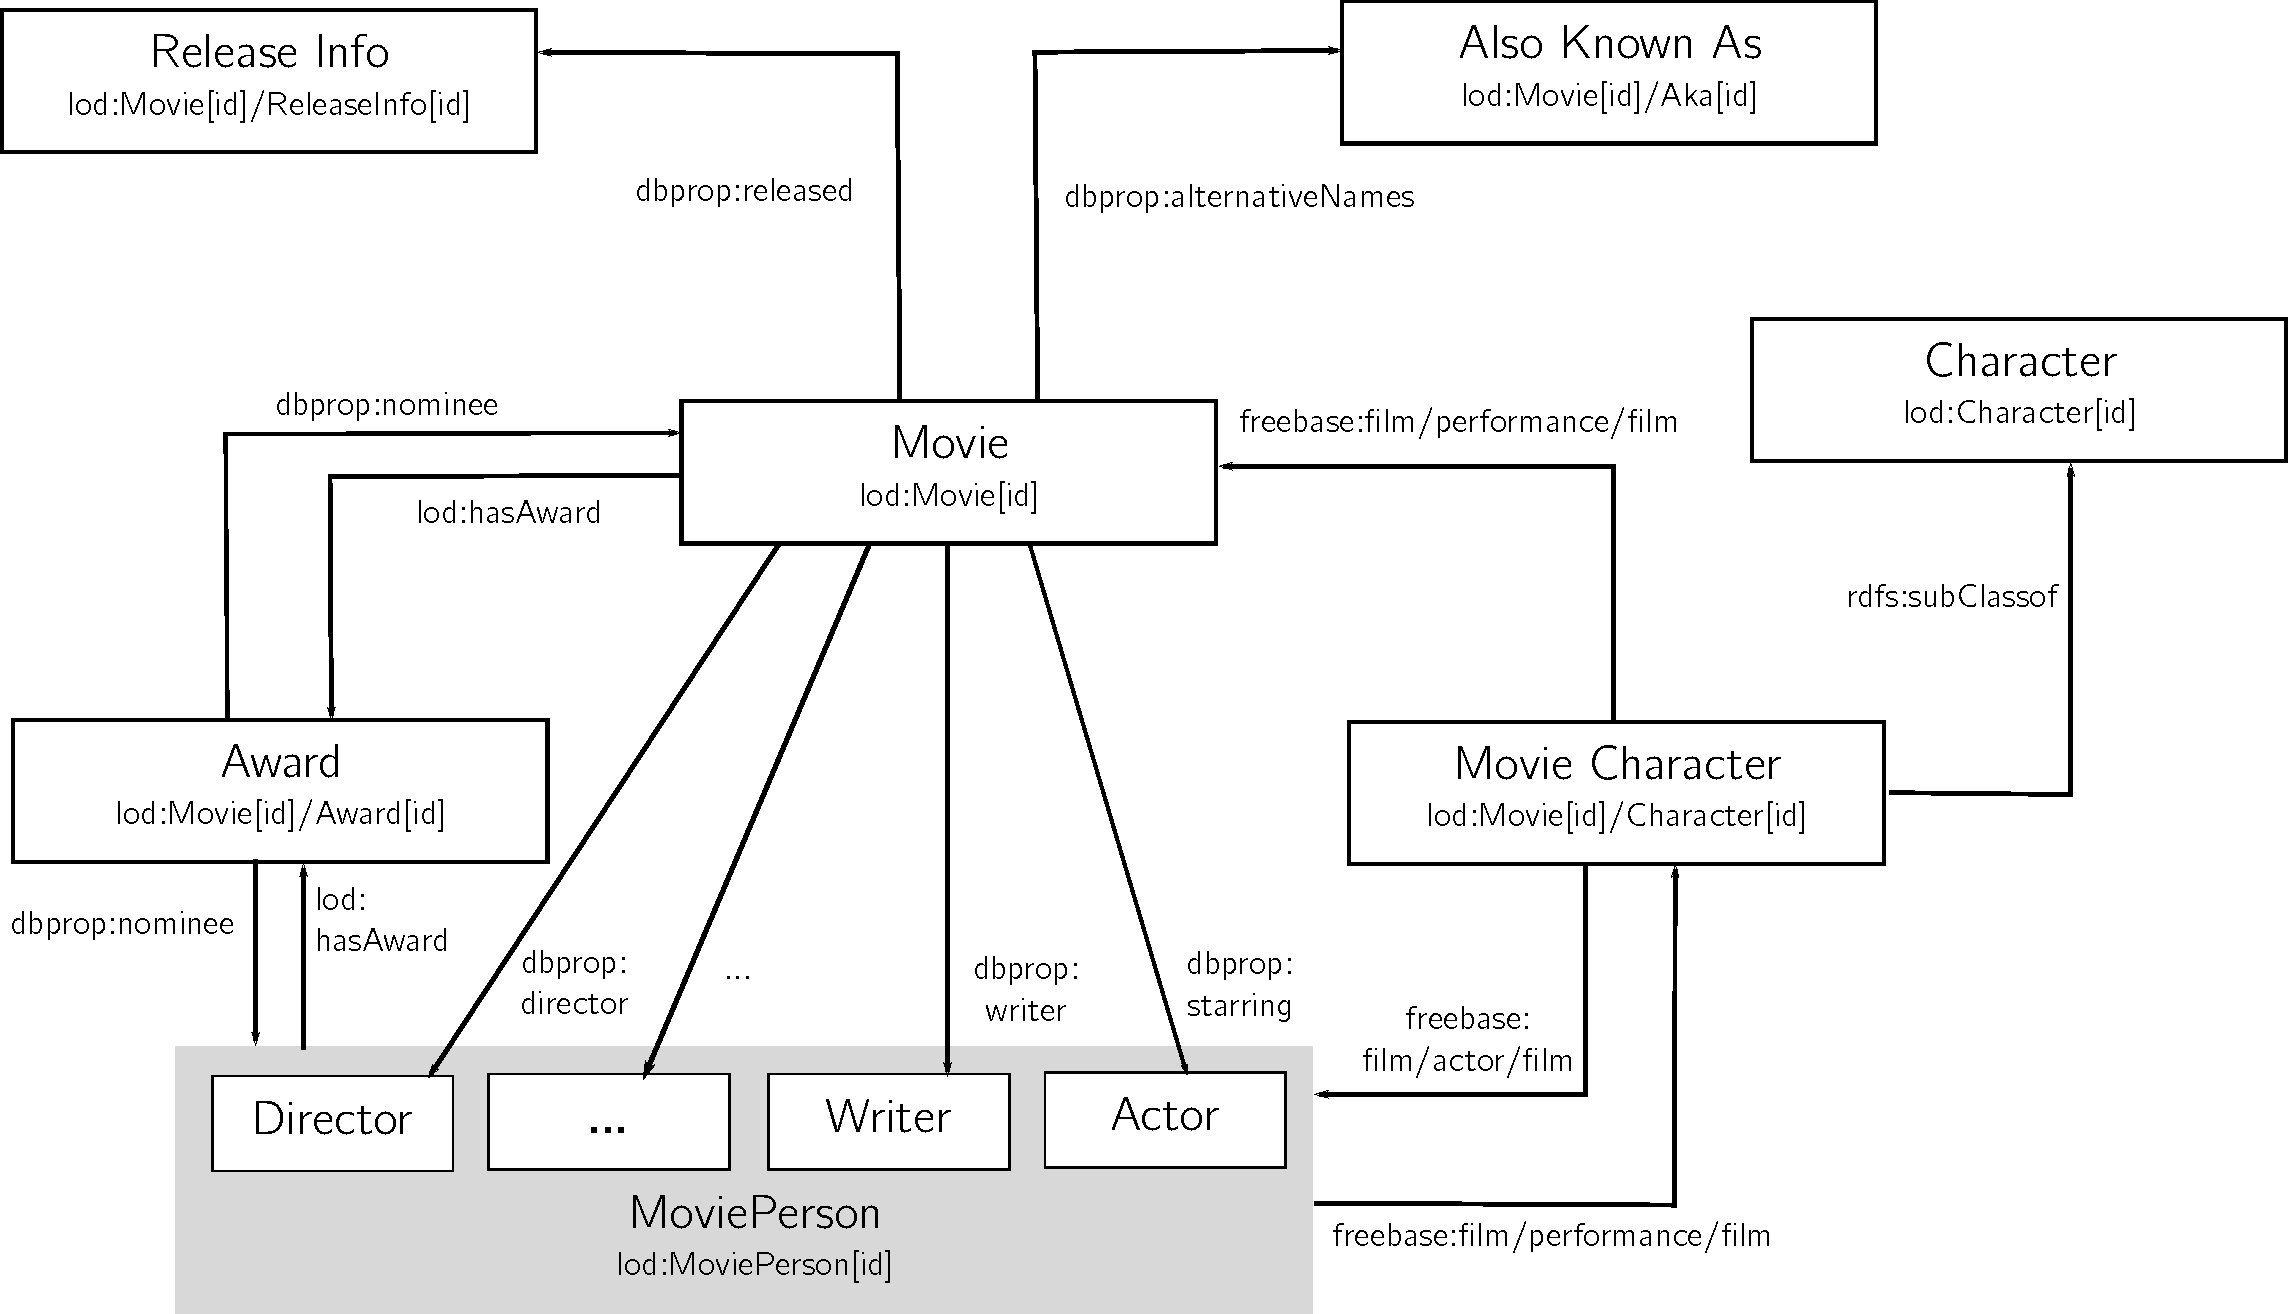
\includegraphics[width=\textwidth]{images/ontology.pdf}
\caption{Ontology}
\label{fig_ontology}
\end{figure}

The naive way to express roles, shown in Figure \ref{fig_ontology}, was one \emph{character} class which was connected to the corresponding movie (via film/performance) and actor (actor or performance).
This meant that a role which exists in multiple movies (e.g. "cleaning lady") would be one resource with an \emph{actor} property for each actor who had ever portrayed this role. 

This approach could cause problems in some cases.
One such case is an actor who played a certain role in an old movie but also appears in the movie's newer remake.
In the remake, they might play a different role while another actor plays their original role. 
An example for this is the movie "Starsky \& Hutch" (2004), which is a remake of the (1970s) television series with the same name.
In the movie, both actors which originally portrayed Starsky and Hutch get a cameo appearance alongside the new cast for their old roles.
With the naive approach, the system could not know who played the Starsky role in the remake, because only references to the movies and the actors are given.

Therefore, an additional class of \emph{MovieCharacter} was introduced.
The resources of this class knows exactly one movie and all actors who played this role in this one movie.
The \emph{MovieCharacter} has a connection, named \emph{Character}, to the \emph{Character} class, which describes the general role.
This means that the \emph{MovieCharacter} in the "Starsky \& Hutch" example is "StarksyStarsky\&Hutch1970" and the \emph{Character} is "Starksy".

%TODO ??More detailed description of diagram??
%TODO ??How many total different entity types, relation types, property types??